\chapter{Introduction} \label{ch:intro}
\section{Motivation}
Occupancy estimation of a given space is an attractive use case of IoT (Internet of Things) devices. Knowing an approximate number of people may help by optimization of HVAC (Heating, Ventilation and Air-condition) consumption in a smart building. At home, a continuous monitoring of dwell time in each room may improve the safety of elder residents. Since the Corona pandemic break out, there has also been a strong demand for monitoring the people number inside a building for social distance controlling.

Many different sensors could be used to sense the number of humans in a given space. \citeauthor{humansense2010survey} \cite{humansense2010survey} has classified the signals presenting into three categories and given their corresponding sensors. Static signals are the intrinsic attributes of a human and are detectable even if the human stays still. Examples in this category are weight (measured by pressure sensor), reflectivity (camera) or emissivity (thermal sensor). Dynamic signals are the activities of a human, such as body movement detected by a ultrasonic sensor \cite{ultrasonic2012doorjamb} or speech detected by a microphone \cite{microphone}. Finally, external traits are the traits of objects carried by a person. A common case is a wearable RFID card \cite{RFID}. Due to the broad use of mobile phones nowadays, Wifi connection activity could also be a good indicator of human occupancy \cite{Wifi}. Beyond the three categories, a coarse estimation of a large amount of people could also be derived from the power consumption, number of lights switched on or the CO2 concentration in a building \cite{CO2}.

Among all sensors, the camera based method is chosen because its capability to detect human in both static/ dynamic scenarios, and the capability to handle complex scenarios with multiple human co-occurrence. An human count estimation by cameras could be obtained either by absolute counting or relative counting. The former method manages to overwatch the whole region of interest by one camera or by merging information from several cameras. The human count at a given time is determined by one single frame using object detection. Therefore, the counting algorithm is independent of camera frame rate as well as the number of people entering/ leaving simultaneously. The relative counting method only monitors the entrance of a room. The final count value is obtained by accumulating the number of entering/ exiting events. A tracking algorithm is required, therefore camera frame rate is critical. And for each frame, the tracking must be done strictly within the time window before the next frame is captured. Besides, when multiple people enter/ exit at the same time the algorithm should still be capable to track correctly.

Our approach is based on a relative counting method because we want to design a general device that is independent of the possible room space. Such a device is sometimes called a doorway turnstile \cite{griffiths2017empirical}.

However, how to monitor the people by a camera in a public space without intruding their privacy poses a challenge to the device design. Due to concerns about privacy violation, RGB-cameras are usually excluded from home surveillance designs \cite{privacyconcerns}. Monitoring through a low-resolution infrared camera may solve the challenge fundamentally. The most remarkable feature of this kind of cameras is that they only have several pixels in vertical and horizontal directions respectively. Sometimes these cameras are referred as thermopile sensors. Thanks to the nature of low-resolution, a person could be detected but the identification of the person is impossible. Without the suspicion of leaking privacy, the monitor device is ideal for an application in public space, but also at home. Moreover, despite the fact that infrared cameras are usually much more expensive than common RGB-cameras, a low-resolution infrared camera is still affordable at the cost of low accuracy and scarce pixels, therefore it is suitable for mass deployment.

In an IoT application, usually a MCU (micro-controller unit) serves as the process unit. A MCU features constraint hardware resources comparing to cloud computation server or common personal computers and smartphones. Beside the low CPU clock rate, a ``large'' MCU can only offer several hundreds KB of memory (SRAM) and several MB of storage (Flash), while a low-end MCU has down to several KB of memory available. One way to bypass the hardware limit is introducing cloud computation, so that the MCU acts as an intermediate handler without processing the data locally, but publishes raw data to a server and receives computational results later. The drawback is the increased network traffic and a higher requirement for a stable network connection. By selecting an adequate microcontroller, we choose to process the collected image data locally to reduce network traffic as well as further minimizing the risk of privacy leakage.

Recently, machine learning (ML) methods play an increasingly critical role in IoT applications. A lot of frameworks and networks has emerged rapidly to achieve the optimal performance within the tiny resource budget of a microcontroller, thus gives the name ``TinyML''. A common workflow of TinyML including exporting the trained model to binary, downloading the model weights to the Flash and allocating an tensor buffer in the memory to store intermediate activations generated by runtime inferencing. The shortage of memory (SRAM) turns out to be the most prominent limit in the deployment of a ML model. It is widely agreed that to reach higher accuracy, a deeper network performs better than a shallow one, but at the cost of a higher peak memory usage. In turn, the memory limit of a microcontroller sets the upper limit of the model accuracy. As one of the most successful research landmarks, \citeauthor{mcunet2020lin} \cite{mcunet2020lin} achieved 61.8\% top-1 accuracy for classification on a microcontroller with 320KB memory and 1MB storage, and the performance drops drastically when latency constraint is considered (to 49.9\% at 5FPS and 40.5\% at 10FPS).

Despite the achievements in ML methods, no model has been developed for short image sequences that is required in our human counting turnstile. The reason could be a higher peak memory consumption due to the demand to store information from multiple images instead of one, and a relative high latency requirement because a human usually passes a doorway within one second. To meet the hardware limit and latency constraint, we turn to traditional computer vision (CV) methods of blob detection \cite{kaspers2011blob}, which drastically cut down the memory usage and process time.

Finally, a balance should be reached between the process capability power consumption. A powerful MCU with higher clock rate can easily meet the latency constraint but drains the battery faster when the same performance can be reached by optimizing the algorithm. Besides, a powerful MCU is also more expensive and increases the budget for mass deployment.

\section{Contribution}
This thesis proposes a human tracking algorithm which is based on traditional CV methods of blob tracking. The algorithm takes a top-view frame sequence of an infrared camera as input and outputs the relative count of the event. The absolute number of people in a room is obtained by accumulating the relative counts. A highlight of the algorithm is its capability to tracking multiple human instances, even when their blob representations merge or split. Several examples are shown in \autoref{fig:cornercases}. Our approach reaches around 95\% accuracy in the test environment and around 80\% accuracy in the real environment. 

We have deployed the algorithm on an ESP32 microcontroller and developed a standalone human counting device that do not need any wire connection to the outside. Communication between the device and a data storage platform is implemented through Wi-Fi and MQTT. The device is powered by a battery therefore it can be detached from the power grid.
\begin{figure}
  \centering
  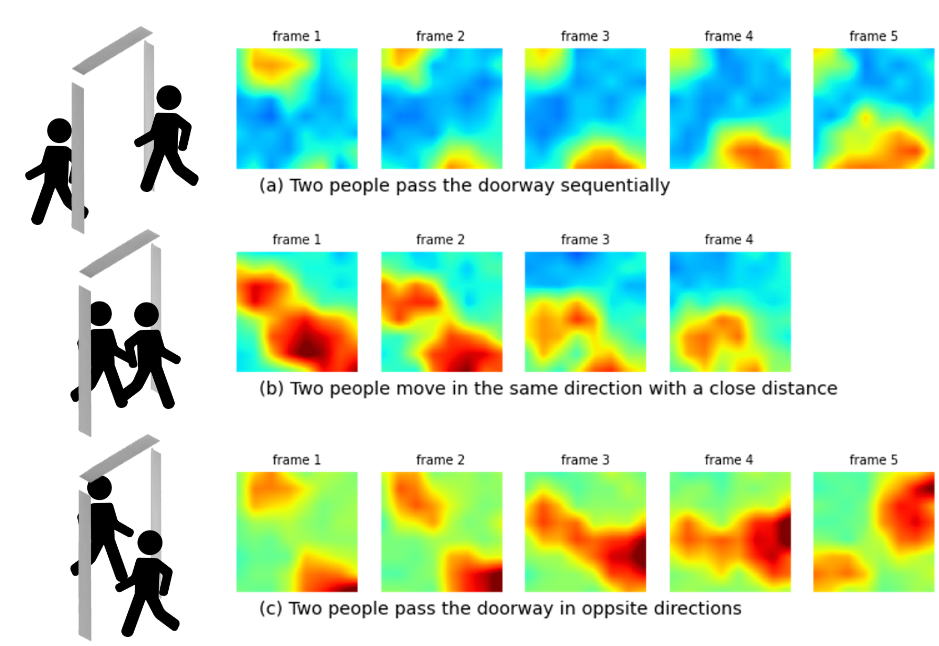
\includegraphics[width=0.85\textwidth]{figures/cornercases.PNG}
  \caption{several corner cases that the proposed algorithm is capable to handle}\label{fig:cornercases}
\end{figure}

\section{Thesis Overview}
In the next chapter, related works will be reviewed. In \Cref{ch:hardware}, the objectives of the design will be described in detail and certain choices of hardware are explained. \Cref{ch:platform} introduces the communication protocol between the end node device and the data centralization platform. The main idea of the proposed algorithm is introduced in \Cref{ch:algorithm}. And \Cref{ch:evaluation} shows the final accuracy of the purposed algorithm based on an eight-days in-situation test.




